\documentclass{article}
\author{Matteo Lucca \& Thorben Finke}
\title{}
\date{}
\usepackage{amsmath}
\parindent 0,5 cm
\usepackage{amssymb}
\usepackage{graphicx}
\usepackage{floatflt}
\usepackage[latin1]{inputenc}
\usepackage{hyperref}
\usepackage{color}

\begin{document}

\subsection*{Exercise 1}
\paragraph{a)} The shower generation after a propagated distance X is $n=X/X_{1/2}$, where $X_{1/2}=X_0 \ln(2)$ is the characteristic length after which the energy is halved and $X_0$ is the characteristic interaction length for pair production and Bremsstrahlung. In the lecture is has been shown that when the shower maximum is reached $n=n_{\rm max}=\ln(E_0/E_{\rm c})/\ln(2)$ so that
\begin{align}
X_{\rm max}=n_{\rm max}X_{1/2}=\frac{\ln(E_0/E_{\rm c})}{\ln(2)}X_0\ln(2)=\ln\left(\frac{E_0}{E_{\rm c}}\right)X_0
\end{align}

\paragraph{b)} With an approximate atomic number of $Z\approx 7.2$ for air, the critical energy becomes
\begin{align}
E_c=\frac{710}{Z+0.92} {\rm MeV}\approx 89  {\rm MeV}
\end{align}
so that (assuming as done in Ex. 4 of Sheet 4 that $X_0=36$ g/cm$^2$) $X_{\rm max}(E_0=1{\rm TeV})=335.4$ g/cm$^2$ and $X_{\rm max}(E_0=30{\rm GeV})=209.1$ g/cm$^2$.

\paragraph{c)}
In the Heitler model 
\begin{align}
R_{\rm el}=\frac{dX_{\rm max}}{d\ln(E_0)}=X_0\frac{d(\ln(E_0)-\ln(E_c))}{d\ln(E_0)}=X_0
\end{align}
so that for and increase in the energy $E_0$ of order $e\approx 2.7$, the maximum length $X_{\rm max}$ increases of a factor $X_0$.

\paragraph{d)}
According to the definitions on the exercise sheet
\begin{align}
X_{\rm max}^{\rm A}=X_{\rm max}^{\rm p}-X_0\ln({\rm A})
\end{align}
with 
\begin{align}
X_{\rm max}^{\rm p}=\lambda_{\rm I}\ln(2)+X_0 \ln\left(\frac{E_0}{6N_\pi E_{\rm c}^{\gamma}}\right)
\end{align}
where $\lambda_{\rm I}$ is the interaction length
\begin{align}
\lambda_{\rm I}=\left(90-9\ln\left(\frac{E_0}{{\rm EeV}}\right)\right)\frac{{\rm g}}{{\rm cm}^2}
\end{align}
and 
\begin{align}
N_\pi=\left(\frac{E_0}{{\rm PeV}}\right)^{1/5}
\end{align}
Putting it all together we obtain that
\begin{align}
\nonumber
X_{\rm max}^{\rm A} & =X_{\rm max}^{\rm p}-X_0\ln({\rm A})= \\
\nonumber
& = \lambda_{\rm I}\ln(2)+X_0 \ln\left(\frac{E_0}{6N_\pi E_{\rm c}^{\gamma}}\right)-X_0\ln({\rm A})= \\
\nonumber
& = \ln(2)\left(90-9\ln\left(\frac{E_0}{{\rm EeV}}\right)\right)\frac{{\rm g}}{{\rm cm}^2}+X_0 \ln\left(\frac{E_0}{6 E_{\rm c}^{\gamma}}\frac{{\rm PeV}^{1/5}}{E_{0}^{1/5}}\right)+ \\ & \nonumber \hspace{0.4 cm}-X_0\ln({\rm A})= \\
\nonumber
& \approx \left[62-6\ln\left(\frac{E_0}{{\rm EeV}}\right)-36\ln(6)+36\ln\left(\frac{E_0}{E_{\rm c}^{\gamma}}\right)+\right. \\ & \nonumber \hspace{0.4 cm}\left.+36\ln\left(\frac{{\rm PeV}^{1/5}}{E_{0}^{1/5}}\right)-36\ln({\rm A})\right]\frac{{\rm g}}{{\rm cm}^2} =\\
\nonumber
& \approx \left\{-2-36\ln({\rm A})+6\left[-\ln\left(\frac{E_0}{{\rm EeV}}\right)+6\ln\left(\frac{E_0}{E_{\rm c}^{\gamma}}\right)+\right.\right. \\ & \nonumber \hspace{0.4 cm}\left.\left.+\frac{6}{5}\ln\left(\frac{{\rm PeV}}{E_{0}}\right)\right]\right\}\frac{{\rm g}}{{\rm cm}^2}=\\
\nonumber
& \approx \left[-2-36\ln({\rm A})+6\ln\left(\frac{10^{18}{\rm eV}}{E_0}\frac{E_{0}^{6}}{(E_{\rm c}^{\gamma})^6}\frac{(10^{15}{\rm eV})^{6/5}}{E_{0}^{6/5}}\right)\right]\frac{{\rm g}}{{\rm cm}^2}=\\
\nonumber
& \approx \left[-2-36\ln({\rm A})+6\ln\left(\frac{E_{0}^{4}10^{36}{\rm eV}^2}{(E_{\rm c}^{\gamma})^6}\right)\right]\frac{{\rm g}}{{\rm cm}^2}=\\
\nonumber
& \approx \left[-2-36\ln({\rm A})+12\ln\left(\frac{E_{0}^{2}{\rm EeV}}{(E_{\rm c}^{\gamma})^3}\right)\right]\frac{{\rm g}}{{\rm cm}^2}
\end{align}
so that 
\begin{align}
c^{\rm A}=\left[-2-36\ln({\rm A})\right]\frac{{\rm g}}{{\rm cm}^2}
\end{align}
and 
\begin{align}
R_{\rm el}=12??
\end{align}
which is independent on A, as to prove. 

\pagebreak
\paragraph{e)}
By plotting $X_{\rm max}$ for photons-, protons- and iron-induced air showers we obtain the following plot:
\begin{figure}[h]
\centering
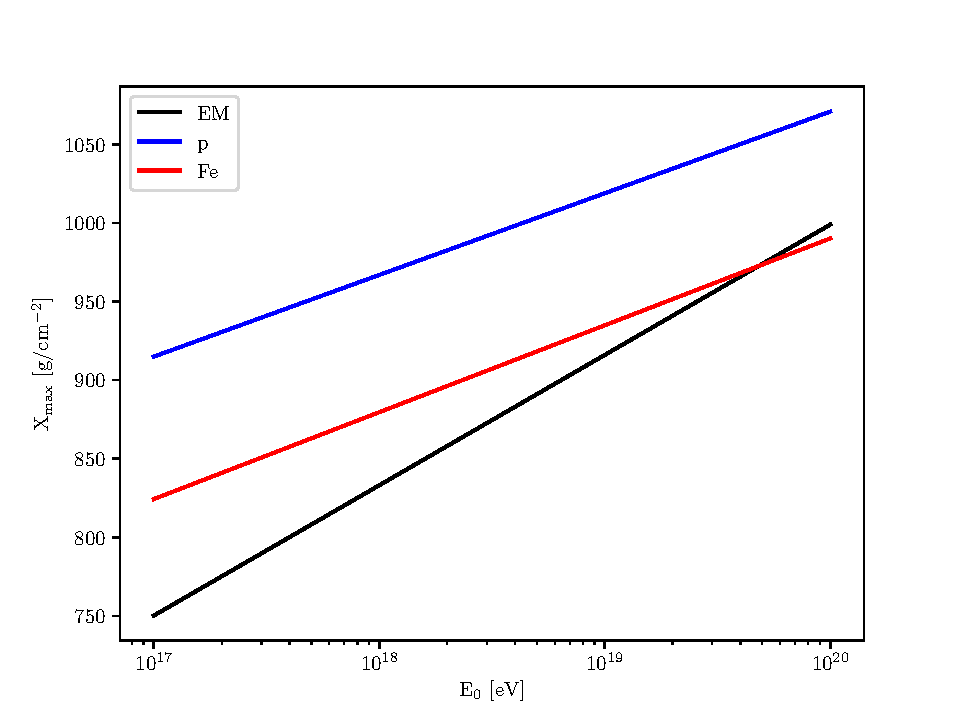
\includegraphics[height=6 cm, width=8 cm]{plot_ex_1e.pdf}
\end{figure}

\paragraph{f)}

\section*{Exercise 2}
\paragraph{a)}
By solving the integral 
\begin{align}
N_{\rm e}(x)=2\pi\int r \rho_{\rm e}(r,x)dr
\end{align}
with 
\begin{align}
\rho_{\rm e}(r,x)=\frac{N_{\rm e}(x)C_1(s)}{r_{\rm s}^{2}}\left(\frac{r}{r_{\rm s}}\right)^{s-2}\left(\frac{r_{\rm s}+r}{r_{\rm s}}\right)^{s-4.5}
\end{align}
one obtains that 
\begin{align}
C_1(s)=\frac{1}{2\pi\int\frac{r}{r_{s}^{2}}\left(\frac{r}{r_{\rm s}}\right)^{s-2}\left(\frac{r_{\rm s}+r}{r_{\rm s}}\right)^{s-4.5}}
\end{align}
For $s=1.25$ we get that $C_1=0.447$.

\paragraph{b)}
According to the lecture notes, the lateral distribution of the particle density for hadronic showers is given by
\begin{align}
\rho(r,x)=\frac{N(x)C_1(s)}{r_{\rm s}^{2}}\left(\frac{r}{r_{\rm s}}\right)^{s-2}\left(\frac{r_{\rm s}+r}{r_{\rm s}}\right)^{s-4.5}\left(1+C_2\left(\frac{r}{r_{\rm s}}\right)^{\delta}\right)
\end{align}
Using $\delta=1$ and $C_2=0.088$ analogously to exercise a) we obtain
\begin{align}
C_1(s)=\frac{1}{2\pi\int\frac{r}{r_{s}^{2}}\left(\frac{r}{r_{\rm s}}\right)^{s-2}\left(\frac{r_{\rm s}+r}{r_{\rm s}}\right)^{s-4.5}\left(1+C_2\frac{r}{r_{\rm s}}\right)}
\end{align}
so that, for $s=1.25$, $C_1=0.403$.

\paragraph{c)}
The following plot displays the lateral distribution for EM (black line) and hadronic (blue line) cascades for $N=10^6$. To define $r_s$ we used the definition (5.173) of the lecture notes to obtain $r_s\approx 8.5$ g cm$^{-2}$ and than we divided it by the air density at sea level ($\rho_0=1.3$ g cm$^{-3}$) to obtain a Moliere radius of 6,5 cm.
\begin{figure}[h]
\centering
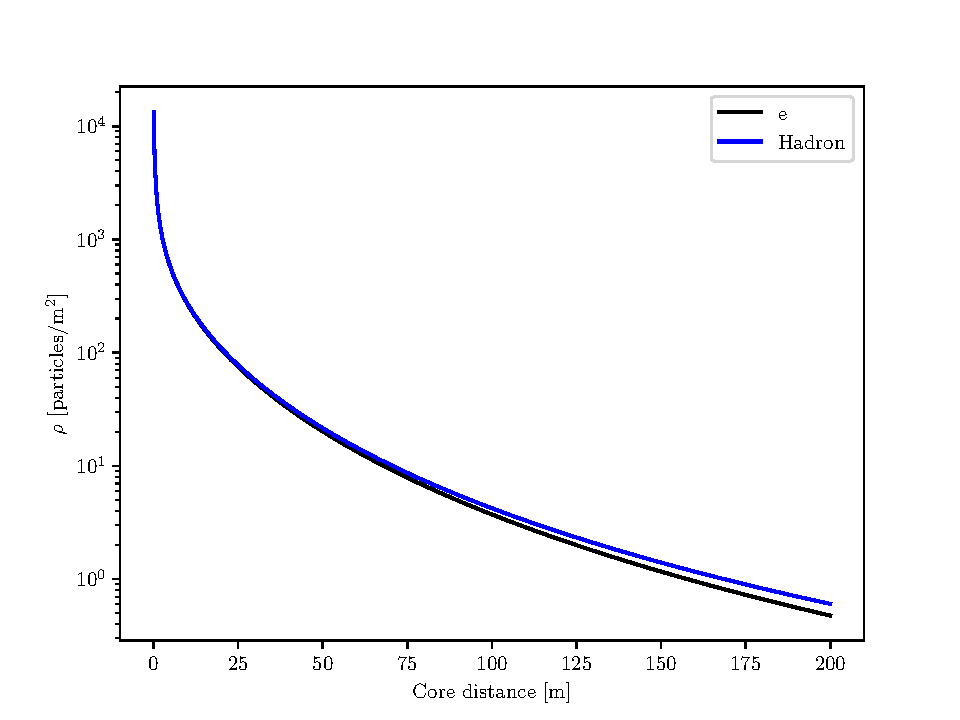
\includegraphics[height=6 cm, width= 8 cm]{plot_ex_2c.pdf}
\label{plot_ex_2c}
\end{figure}
\\* It is possible to observe a deviation for large distances from the core, where the density of EM cascades decreases faster than the density of hadronic cascades. This behavior could be explained with the fact that "hadronic decay particles typically carry larger transversal momenta than EM particles" so that "the transversal extension of hadronic cascades is larger" (Lecture notes p. 109) and with it also the density for very large distances from the shower core. 

\paragraph{d)}
As possible to observe in Fig. \ref{plot_ex_2c}, a density of 1 particle per m$^2$ is reached at a distance from the shower core of $\approx$ 165 m.

\section*{Exercise 3}
\paragraph{a)}
By using the data from the previous exercise, we obtain the following plot. 
\pagebreak
\begin{figure}[h]
\centering
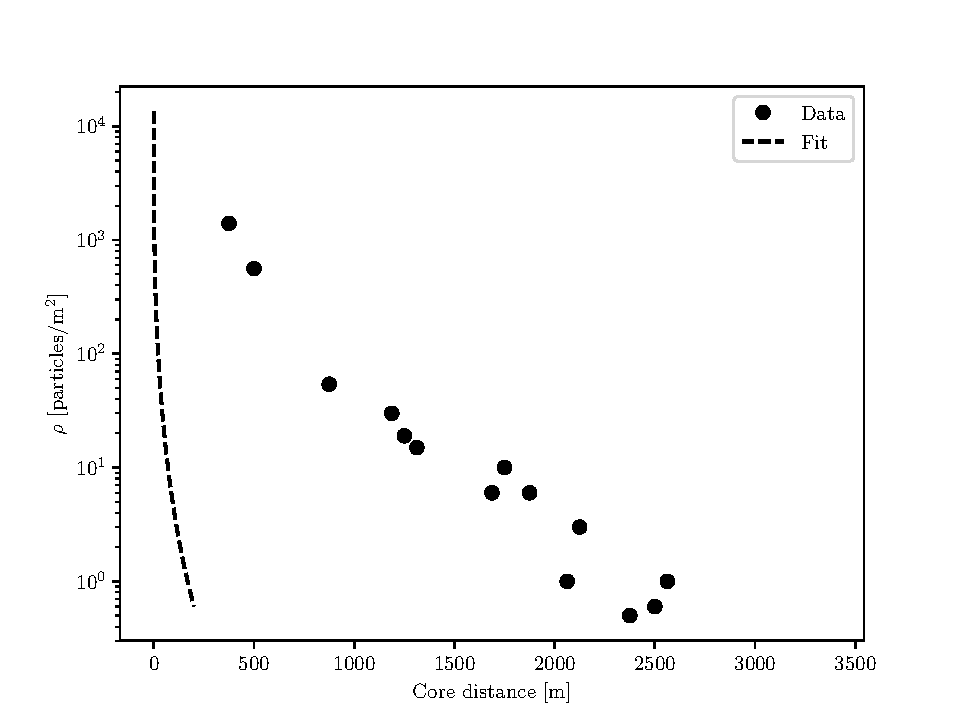
\includegraphics[height=6 cm, width= 8 cm]{plot_ex_3a_1.pdf}
\end{figure}
\\* From the figure it is clear that the number of particle must be higher than the $1\times 10^6$ assumed before.

\paragraph{b)}
By increasing the number of particle to $7\times 10^9$ we obtain the following (more realistic) result. 
\begin{figure}[h]
\centering
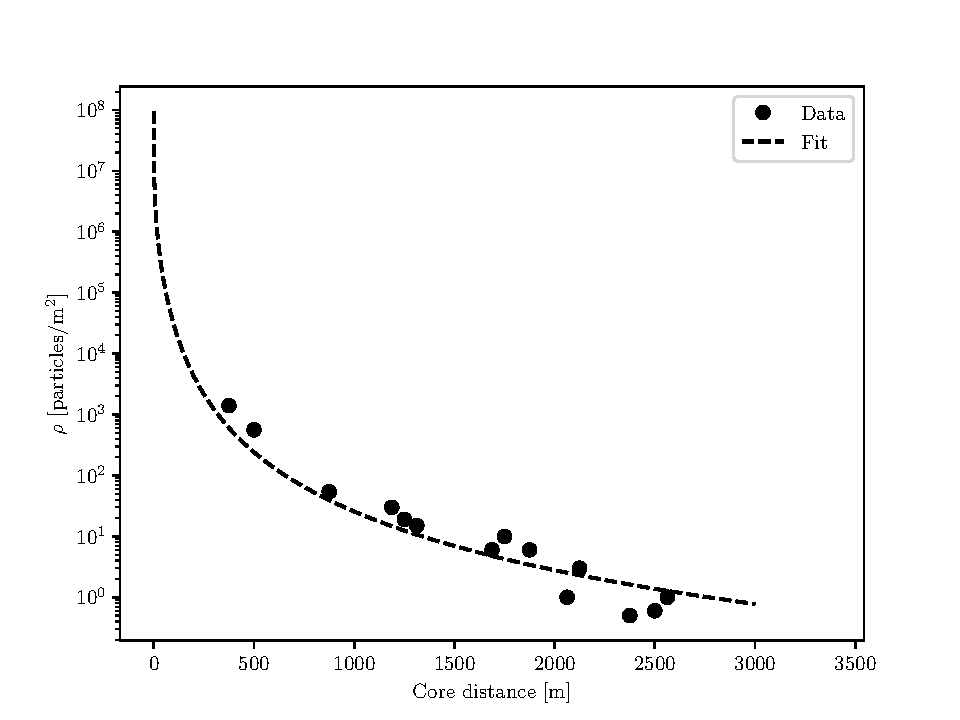
\includegraphics[height=6 cm, width= 8 cm]{plot_ex_3a_2.pdf}
\end{figure}

\paragraph{c)}
Assuming that approximately between 0.1\% and 1\% of the particles reaching ground are muons, i.e. between $7\times 10^6$ and $7\times 10^7$, then according to Fig. 5.128 of the lecture notes (assuming an energy threshold of 1 GeV) the primary energy of the event is approximately between $1\times 10^{18}$ and $1\times 10^{19}$ eV.

\subsection*{Exercise 4}
\paragraph{a)}
According to Huygens' principle each point of a wavefront is source of a elementary wave. 
In the graphic below it is shown how a particle moves from left to right and emits light at each position (shown are just a few examples). 
The resulting wavefront is thus the upper line, tangent to all elementary waves. \\
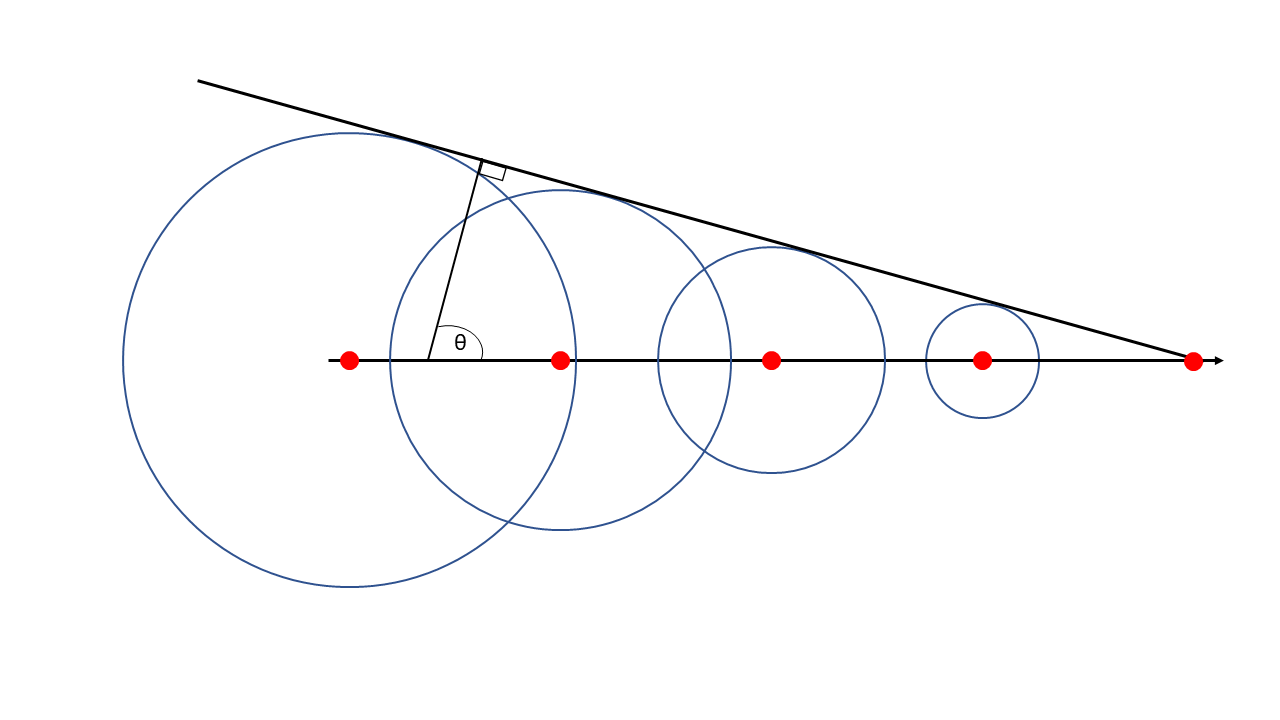
\includegraphics[width=\textwidth]{exercise4.png}\\
Here one can see that 
\begin{align*}
cos(\theta) = \frac{distance\ of\ light}{distance\ of\ particle} = \frac{c't}{\beta c t} = \frac{1}{\beta n}.
\end{align*}
In the last step it is used that the speed of light in medium is given by $c' = c / n$, where n is the refractive index of the medium.

\paragraph{b)}
For relativistic particles - $\beta \approx 1$ - the opening angle for water is $41.30^\circ$ and for $1.38^\circ0$.

\paragraph{c)}
To induce Cherenkov light the particles' speed needs to be higher than the speed of light in the medium. For water that is $c' = c/n < \beta c \rightarrow 1/n < \beta$.
From relativistic kinematics one gets in natural units ($c=1$)
\begin{align*}
E_{kin} = E - E_0 = (\gamma - 1) m_0
\end{align*}
\end{document}
